% ─────────────────────────────────────────────────────────────────────
%  My Musical Mind — A Compositional Overview
%  For Guang Yang — March 2026
%  Amaç Erdem
% ─────────────────────────────────────────────────────────────────────
\documentclass[10pt,a4paper]{article}

\usepackage[margin=2cm, top=1.8cm, bottom=2cm]{geometry}
\usepackage[T1]{fontenc}
\usepackage{palatino}
\usepackage{microtype}
\usepackage{titlesec}
\usepackage{enumitem}
\usepackage{booktabs}
\usepackage{multicol}
\usepackage{xcolor}
\usepackage{tikz}
\usetikzlibrary{positioning, calc, shapes.geometric, fit, backgrounds, arrows}
\usepackage{pgfplots}
\pgfplotsset{compat=1.18}
\usepackage{tcolorbox}
\tcbuselibrary{skins,breakable}
\usepackage{fancyhdr}
\usepackage{hyperref}

% ── Colours ───────────────────────────────────────────────────────────
\definecolor{deep}{HTML}{2C3E6B}
\definecolor{accent}{HTML}{8B5CF6}
\definecolor{warm}{HTML}{C2785C}
\definecolor{sage}{HTML}{4A7C6F}
\definecolor{gold}{HTML}{B8860B}
\definecolor{rose}{HTML}{9E4A6C}
\definecolor{sky}{HTML}{5B9BD5}
\definecolor{mist}{HTML}{F7F5F2}
\definecolor{stone}{HTML}{9CA3AF}
\definecolor{alch}{HTML}{9333EA}
\definecolor{arch}{HTML}{2563EB}
\definecolor{expl}{HTML}{22C55E}
\definecolor{anch}{HTML}{F59E0B}
\definecolor{kine}{HTML}{F97316}
\hypersetup{colorlinks=true, linkcolor=deep, urlcolor=accent, citecolor=warm}

% ── Typography ────────────────────────────────────────────────────────
\titleformat{\section}{\Large\bfseries\sffamily\color{deep}}{}{0em}{}[\vspace{-3pt}{\color{deep!25}\rule{\textwidth}{0.4pt}}]
\titleformat{\subsection}{\normalsize\bfseries\sffamily\color{accent!80!black}}{}{0em}{}
\titlespacing*{\section}{0pt}{10pt}{6pt}
\titlespacing*{\subsection}{0pt}{8pt}{3pt}

\pagestyle{fancy}
\fancyhf{}
\renewcommand{\headrulewidth}{0pt}
\fancyfoot[C]{\color{stone}\sffamily\small \thepage\;/\;5}

\setlength{\parskip}{3pt}
\setlength{\parindent}{0pt}
\setlist{nosep, leftmargin=1.2em}

\newtcolorbox{introbox}[1][]{
  enhanced, colback=mist, colframe=deep!20,
  boxrule=0.4pt, arc=4pt, left=10pt, right=10pt, top=8pt, bottom=8pt,
  fonttitle=\sffamily\bfseries\color{deep}, title=#1
}

\newtcolorbox{accentbox}[1][]{
  enhanced, colback=accent!4, colframe=accent!25,
  boxrule=0.4pt, arc=3pt, left=8pt, right=8pt, top=6pt, bottom=6pt,
  fonttitle=\sffamily\bfseries\small\color{accent!80!black}, title=#1
}

% ══════════════════════════════════════════════════════════════════════
\begin{document}

% ── TITLE ─────────────────────────────────────────────────────────────
\begin{center}
  \vspace*{4pt}
  {\fontsize{24}{28}\selectfont\sffamily\bfseries\color{deep}
   My Musical Mind}\\[5pt]
  {\fontsize{11}{14}\selectfont\sffamily\color{accent!80!black}
   Who Are You as a Listener?}\\[14pt]
  {\normalsize\sffamily Ama\c{c} Erdem\quad$\cdot$\quad For Guang Yang\quad$\cdot$\quad March 2026}
\end{center}

\vspace{8pt}

\begin{introbox}
\begin{multicols}{2}
\small
You know you and I listen to the same quartet differently. You hear the counterpoint; I hear the timbral blend. You lean into the dissonance; I crave the resolution. We both love the piece---but we love it for different reasons.

\smallskip
What if there was a way to \emph{see} those differences? Not as genre labels (``you like jazz'') but as cognitive fingerprints---the actual dimensions of how your ear engages with sound?

\columnbreak

\textbf{My Musical Mind} (M$^3$) is an interactive music discovery platform that maps your listening into a \textbf{six-dimensional cognitive profile}, assigns you one of \textbf{24 musical personas}, and lets that identity \textbf{evolve} as you discover new music. Behind it sits \textbf{Musical Intelligence}---a 131-belief model of musical cognition grounded in 448 studies---but M$^3$ is what you touch: a living portrait of \emph{who you are} as a listener.

\end{multicols}
\end{introbox}

% ══════════════════════════════════════════════════════════════════════
%  PAGE 1 — THE SIX DIMENSIONS
% ══════════════════════════════════════════════════════════════════════
\section{Your Listening Genome: Six Dimensions}

\vspace{2pt}

\begin{multicols}{2}

When you import a playlist, M$^3$ analyses your listening across six perceptual dimensions---not genre tags, but how your \emph{ear and mind} engage with sound:

\vspace{6pt}

\begin{center}
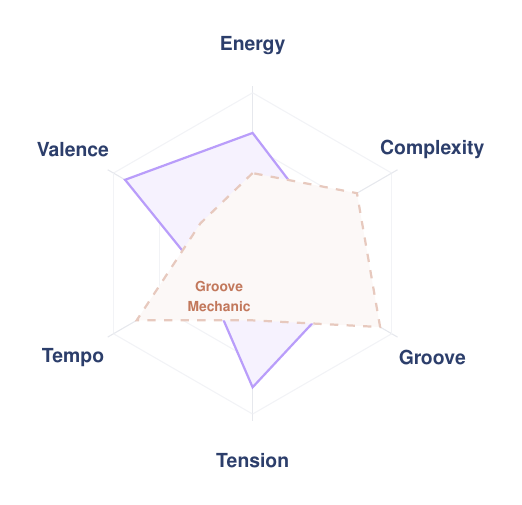
\begin{tikzpicture}[scale=0.85]
  % Grid
  \foreach \i/\lab in {0/Energy, 60/Valence, 120/Tempo, 180/Tension, 240/Groove, 300/Complexity} {
    \draw[deep!12] (0,0) -- (\i+90:2.5cm);
    \node[font=\sffamily\scriptsize\bfseries, text=deep] at (\i+90:3.1cm) {\lab};
    \foreach \r in {0.8,1.6,2.4}
      \draw[deep!6] (\i+90:\r) -- (\i+90+60:\r);
  }
  % Persona shape
  \draw[thick, accent!60, fill=accent!8]
    (90:1.8) -- (150:2.2) -- (210:0.8) -- (270:2.0) -- (330:1.4) -- (30:1.1) -- cycle;
  \node[font=\sffamily\tiny\color{accent}, align=center] at (0.3,0.3) {\textbf{Tension}\\[-1pt]\textbf{Architect}};
  % Ghost
  \draw[thick, warm!40, fill=warm!5, dashed]
    (90:1.2) -- (150:0.9) -- (210:2.0) -- (270:1.0) -- (330:2.2) -- (30:1.8) -- cycle;
  \node[font=\sffamily\tiny\color{warm}] at (-0.5,-0.5) {\textbf{Groove}};
  \node[font=\sffamily\tiny\color{warm}] at (-0.5,-0.8) {\textbf{Mechanic}};
\end{tikzpicture}
\end{center}

{\scriptsize\color{stone} Two listeners, same concert. One drawn to harmonic tension (purple); the other to rhythmic groove (orange). M$^3$ makes the difference visible.}

\columnbreak

\vspace{6pt}

{\small
\begin{tabular}{@{}p{1.8cm}p{5cm}@{}}
  \toprule
  \textbf{\sffamily Dimension} & \textbf{\sffamily What It Measures} \\
  \midrule
  \textcolor{rose}{\sffamily\bfseries Energy} &
    Intensity, arousal. Powerful, loud music vs.\ quiet, calm. How much does the sound \emph{push} you? \\[4pt]
  \textcolor{sky}{\sffamily\bfseries Valence} &
    Emotional tone. Bright and exhilarating vs.\ dark and melancholic. The \emph{emotional colour} of what you seek. \\[4pt]
  \textcolor{kine}{\sffamily\bfseries Tempo} &
    Perceived pace. Fast, driving music vs.\ slow, spacious breathing. \\[4pt]
  \textcolor{alch}{\sffamily\bfseries Tension} &
    Attraction to dissonance, suspense, build-ups. The unresolved dominant seventh. \\[4pt]
  \textcolor{sage}{\sffamily\bfseries Groove} &
    Rhythmic engagement. Entrainment, syncopation, physical momentum. The body's response. \\[4pt]
  \textcolor{arch}{\sffamily\bfseries Complexity} &
    Structural density. Layered counterpoint vs.\ a single melody. \\
  \bottomrule
\end{tabular}
}

\vspace{6pt}

These six values form your \textbf{Listening Genome}---a cognitive fingerprint that describes not \emph{what} you listen to, but \emph{how} you listen.

\end{multicols}

\newpage

% ══════════════════════════════════════════════════════════════════════
%  PAGE 2 — THE 24 PERSONAS & 5 FAMILIES
% ══════════════════════════════════════════════════════════════════════
\section{24 Personas, Five Families}

\vspace{2pt}

Your 6D profile maps to one of \textbf{24 listening personas}, grouped into five \textbf{Neural Families}. Each family represents a fundamentally different way of engaging with sound---and each persona is a specific point in that family's cognitive landscape.

\vspace{6pt}

% ── Family Overview ──────────────────────────────────────────────────

\begin{center}
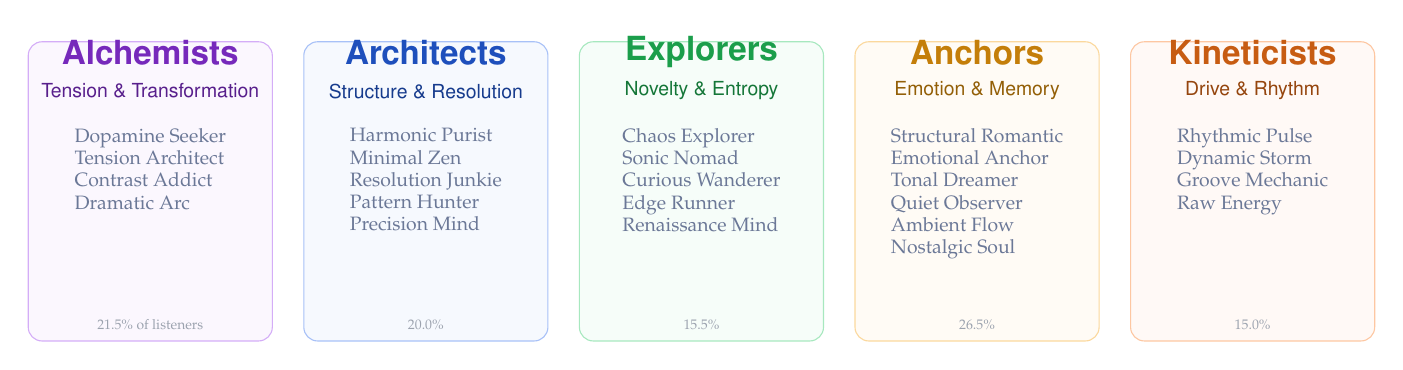
\begin{tikzpicture}[
  fam/.style={draw=#1!40, rounded corners=5pt, minimum width=3.1cm,
              minimum height=3.8cm, fill=#1!4, align=center},
  ftit/.style={font=\sffamily\bfseries\color{#1!80!black}},
  fper/.style={font=\scriptsize\color{deep!70}, align=left}
]

  \node[fam=alch] (a) at (0,0) {};
  \node[ftit=alch] at ([yshift=-4pt]a.north) {\large Alchemists};
  \node[font=\scriptsize\sffamily\color{alch!60!black}] at ([yshift=-18pt]a.north) {Tension \& Transformation};
  \node[fper, anchor=north] at ([yshift=-28pt]a.north) {
    Dopamine Seeker\\Tension Architect\\Contrast Addict\\Dramatic Arc
  };
  \node[font=\tiny\color{stone}] at ([yshift=6pt]a.south) {21.5\% of listeners};

  \node[fam=arch] (b) at (3.5,0) {};
  \node[ftit=arch] at ([yshift=-4pt]b.north) {\large Architects};
  \node[font=\scriptsize\sffamily\color{arch!60!black}] at ([yshift=-18pt]b.north) {Structure \& Resolution};
  \node[fper, anchor=north] at ([yshift=-28pt]b.north) {
    Harmonic Purist\\Minimal Zen\\Resolution Junkie\\Pattern Hunter\\Precision Mind
  };
  \node[font=\tiny\color{stone}] at ([yshift=6pt]b.south) {20.0\%};

  \node[fam=expl] (c) at (7,0) {};
  \node[ftit=expl] at ([yshift=-4pt]c.north) {\large Explorers};
  \node[font=\scriptsize\sffamily\color{expl!60!black}] at ([yshift=-18pt]c.north) {Novelty \& Entropy};
  \node[fper, anchor=north] at ([yshift=-28pt]c.north) {
    Chaos Explorer\\Sonic Nomad\\Curious Wanderer\\Edge Runner\\Renaissance Mind
  };
  \node[font=\tiny\color{stone}] at ([yshift=6pt]c.south) {15.5\%};

  \node[fam=anch] (d) at (10.5,0) {};
  \node[ftit=anch] at ([yshift=-4pt]d.north) {\large Anchors};
  \node[font=\scriptsize\sffamily\color{anch!60!black}] at ([yshift=-18pt]d.north) {Emotion \& Memory};
  \node[fper, anchor=north] at ([yshift=-28pt]d.north) {
    Structural Romantic\\Emotional Anchor\\Tonal Dreamer\\Quiet Observer\\Ambient Flow\\Nostalgic Soul
  };
  \node[font=\tiny\color{stone}] at ([yshift=6pt]d.south) {26.5\%};

  \node[fam=kine] (e) at (14,0) {};
  \node[ftit=kine] at ([yshift=-4pt]e.north) {\large Kineticists};
  \node[font=\scriptsize\sffamily\color{kine!60!black}] at ([yshift=-18pt]e.north) {Drive \& Rhythm};
  \node[fper, anchor=north] at ([yshift=-28pt]e.north) {
    Rhythmic Pulse\\Dynamic Storm\\Groove Mechanic\\Raw Energy
  };
  \node[font=\tiny\color{stone}] at ([yshift=6pt]e.south) {15.0\%};

\end{tikzpicture}
\end{center}

\vspace{4pt}

\begin{multicols}{2}

\subsection{How Is Your Persona Chosen?}

When you import a playlist, the system analyses your tracks and produces your 6D genome. Each of the 24 personas has a \textbf{canonical 6D fingerprint}---for example, the \textcolor{alch}{\textbf{Tension Architect}} sits at tension\,=\,0.92 (very high) with moderate complexity and low energy.

Your persona is the closest match in 6D Euclidean space:

\begin{center}
\fbox{\small\sffamily persona = argmin$_p$\;$\|$\,your genes $-$ persona$_p$ genes\,$\|$}
\end{center}

\smallskip
This isn't genre labelling. Two people who both ``like classical'' might be a \textcolor{arch}{\textbf{Harmonic Purist}} (drawn to intervallic beauty) and a \textcolor{alch}{\textbf{Dramatic Arc}} (drawn to large-scale tension)---the same repertoire, entirely different cognitive signatures.

\columnbreak

\subsection{Personas Evolve}

Your persona is not fixed. It shifts as your listening deepens. A composer spending a summer immersed in spectralism might drift from Architect to Explorer. A season of Brazilian rhythm might pull toward Kineticist.

\smallskip
M$^3$ tracks this evolution through \textbf{12 developmental levels}:

\vspace{4pt}
{\small
\begin{tabular}{@{}cl@{}}
  \toprule
  \textbf{Level} & \textbf{Stage} \\
  \midrule
  1--4 & Embryonic $\to$ Infant (sensory awakening) \\
  5--8 & Toddler $\to$ Child (pattern recognition) \\
  9--10 & Adolescent (social awareness) \\
  11--12 & Adult $\to$ Elder (meta-awareness) \\
  \bottomrule
\end{tabular}
}

\vspace{4pt}

Each level reveals new cognitive observations about your listening---deeper insights that emerge only after sustained engagement.

\end{multicols}

\newpage

% ══════════════════════════════════════════════════════════════════════
%  PAGE 3 — THE EXPERIENCE
% ══════════════════════════════════════════════════════════════════════
\section{The Experience: Discover, Play, Connect}

\vspace{4pt}

\begin{center}
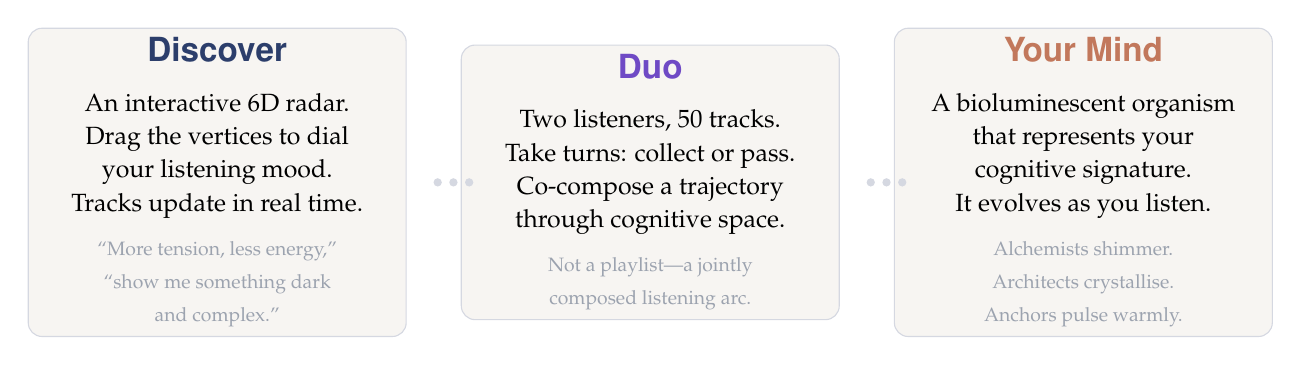
\begin{tikzpicture}[
  phase/.style={draw=deep!20, rounded corners=5pt, minimum width=4.8cm,
                minimum height=3.2cm, fill=mist, align=center}
]

  \node[phase] (disc) at (0,0) {
    {\large\bfseries\sffamily\color{deep} Discover}\\[6pt]
    {\small An interactive 6D radar.}\\
    {\small Drag the vertices to dial}\\
    {\small your listening mood.}\\
    {\small Tracks update in real time.}\\[4pt]
    {\scriptsize\color{stone} ``More tension, less energy,''}\\
    {\scriptsize\color{stone} ``show me something dark}\\
    {\scriptsize\color{stone} and complex.''}
  };

  \node[phase] (duo) at (5.5,0) {
    {\large\bfseries\sffamily\color{accent!80!black} Duo}\\[6pt]
    {\small Two listeners, 50 tracks.}\\
    {\small Take turns: collect or pass.}\\
    {\small Co-compose a trajectory}\\
    {\small through cognitive space.}\\[4pt]
    {\scriptsize\color{stone} Not a playlist---a jointly}\\
    {\scriptsize\color{stone} composed listening arc.}
  };

  \node[phase] (mind) at (11,0) {
    {\large\bfseries\sffamily\color{warm} Your Mind}\\[6pt]
    {\small A bioluminescent organism}\\
    {\small that represents your}\\
    {\small cognitive signature.}\\
    {\small It evolves as you listen.}\\[4pt]
    {\scriptsize\color{stone} Alchemists shimmer.}\\
    {\scriptsize\color{stone} Architects crystallise.}\\
    {\scriptsize\color{stone} Anchors pulse warmly.}
  };

  % Connecting dots
  \foreach \x in {2.8, 3.0, 3.2} \fill[deep!20] (\x,0) circle (1.5pt);
  \foreach \x in {8.3, 8.5, 8.7} \fill[deep!20] (\x,0) circle (1.5pt);

\end{tikzpicture}
\end{center}

\vspace{8pt}

\begin{multicols}{2}

\subsection{The Discovery Radar}

The heart of M$^3$ is a hexagonal radar with six draggable vertices---one per dimension. Pull \textbf{Tension} high and \textbf{Energy} low, and you'll hear dark, suspenseful, intimate music. Max out \textbf{Groove} and \textbf{Tempo}, and the feed shifts to driving, danceable tracks.

This isn't search. It's \emph{compositional navigation}---you're sculpting the acoustic space you want to inhabit, and M$^3$ finds music that lives there.

\subsection{The Duo Mode}

Two listeners enter a shared listening space. From a pool of 50 tracks, they alternate: each turn, you hear a track and choose to \textbf{collect} or \textbf{pass}. After 12 collected tracks, a co-created trajectory emerges.

\begin{center}
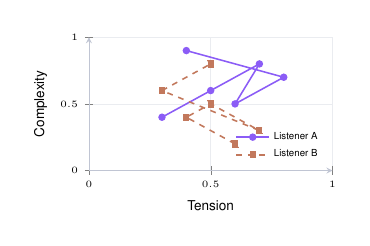
\begin{tikzpicture}[scale=0.7]
  \begin{axis}[
    width=6cm, height=4cm,
    xlabel={\scriptsize\sffamily Tension},
    ylabel={\scriptsize\sffamily Complexity},
    xmin=0, xmax=1, ymin=0, ymax=1,
    xtick={0,0.5,1}, ytick={0,0.5,1},
    grid=major, grid style={deep!10},
    tick label style={font=\tiny\sffamily},
    label style={font=\tiny\sffamily},
    axis lines=left,
    axis line style={deep!30},
    legend style={font=\sffamily\tiny, at={(0.98,0.02)}, anchor=south east, draw=none, fill=none},
  ]
    \addplot[thick, accent, mark=*, mark size=1.5pt] coordinates {
      (0.3,0.4) (0.5,0.6) (0.7,0.8) (0.6,0.5) (0.8,0.7) (0.4,0.9)};
    \addlegendentry{Listener A}
    \addplot[thick, warm, mark=square*, mark size=1.5pt, dashed] coordinates {
      (0.6,0.2) (0.4,0.4) (0.5,0.5) (0.7,0.3) (0.3,0.6) (0.5,0.8)};
    \addlegendentry{Listener B}
  \end{axis}
\end{tikzpicture}
\end{center}

{\scriptsize\color{stone} Two listeners converging through Tension--Complexity space. Where their trajectories cross: aesthetic agreement. Where they diverge: creative dialogue.}

\columnbreak

\subsection{The Organism}

Each persona has a living visual form---a bioluminescent organism rendered in WebGL. Its morphology expresses its family:

\vspace{4pt}
{\small
\begin{tabular}{@{}p{2cm}p{4.5cm}@{}}
  \toprule
  \textbf{\sffamily Family} & \textbf{\sffamily Visual Character} \\
  \midrule
  \textcolor{alch}{\sffamily Alchemists} &
    Volatile, electric, jagged. Shimmering with internal tension. \\[3pt]
  \textcolor{arch}{\sffamily Architects} &
    Crystalline, angular, faceted. Precise geometric forms. \\[3pt]
  \textcolor{expl}{\sffamily Explorers} &
    Fluid, chaotic, morphing. Constantly reshaping. \\[3pt]
  \textcolor{anch}{\sffamily Anchors} &
    Organic, smooth, warm. Pulsing with inner light. \\[3pt]
  \textcolor{kine}{\sffamily Kineticists} &
    Rhythmic, orbital, pulsing. Energy in periodic motion. \\
  \bottomrule
\end{tabular}
}

\vspace{6pt}

As you level up, the organism gains visual complexity---new limbs, deeper colour saturation, more intricate patterns. By Level 12, it's a full expression of your accumulated listening identity.

\subsection{The Resonance Field}

A real-time visualisation of all listeners currently online. Each is a glowing organism in a shared 3D space---hover to see their persona, level, and preferred genres. Find someone interesting? Enter a Duo.

\end{multicols}

\newpage

% ══════════════════════════════════════════════════════════════════════
%  PAGE 4 — WHAT'S BEHIND IT: MI CONNECTION
% ══════════════════════════════════════════════════════════════════════
\section{What Powers It: Musical Intelligence}

\vspace{2pt}

\begin{multicols}{2}

The six dimensions are not arbitrary. They emerge from \textbf{Musical Intelligence (MI)}---a computational model of how the human mind processes music, built on 448 published studies in music cognition and auditory neuroscience.

\subsection{From Sound to Meaning}

MI listens to audio and tracks 131 simultaneous ``beliefs'' about the music---not frequencies or spectrograms, but \emph{compositional qualities}:

\begin{itemize}[itemsep=3pt]
  \item \textbf{Is this harmony stable or unstable?} Consonance hierarchies following Sethares, Plomp--Levelt, Krumhansl--Kessler.
  \item \textbf{What should come next?} Melodic, harmonic, and rhythmic expectancy at multiple temporal scales.
  \item \textbf{What grabbed my attention?} Novelty detection, foreground--background segregation.
  \item \textbf{Does this remind me of something?} Familiarity modulation, episodic memory binding.
  \item \textbf{How does this feel?} Valence--arousal mapping, nostalgia, emotional contagion.
  \item \textbf{Does my body want to move?} Beat entrainment, phase locking, syncopation response.
  \item \textbf{Why is this moment beautiful?} Prediction error aggregated across all dimensions.
\end{itemize}

\columnbreak

\subsection{How MI Becomes Your Genome}

MI's 131 beliefs condense into the same \textbf{6D space} that defines your persona:

\vspace{6pt}

\begin{center}
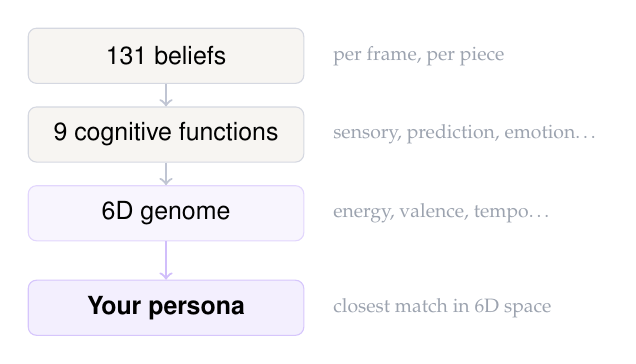
\begin{tikzpicture}[
  bx/.style={draw=deep!20, rounded corners=3pt, fill=mist,
             minimum width=3.5cm, minimum height=0.7cm,
             font=\sffamily\small, align=center}
]
  \node[bx] (mi) at (0,3.2) {131 beliefs};
  \node[bx] (agg) at (0,2.2) {9 cognitive functions};
  \node[bx, fill=accent!6, draw=accent!25] (gene) at (0,1.2) {6D genome};
  \node[bx, fill=accent!10, draw=accent!35] (per) at (0,0) {\textbf{Your persona}};

  \draw[->, thick, draw=deep!30] (mi) -- (agg);
  \draw[->, thick, draw=deep!30] (agg) -- (gene);
  \draw[->, thick, draw=accent!40] (gene) -- (per);

  \node[font=\scriptsize\color{stone}, anchor=west] at (2,3.2) {per frame, per piece};
  \node[font=\scriptsize\color{stone}, anchor=west] at (2,2.2) {sensory, prediction, emotion\ldots};
  \node[font=\scriptsize\color{stone}, anchor=west] at (2,1.2) {energy, valence, tempo\ldots};
  \node[font=\scriptsize\color{stone}, anchor=west] at (2,0) {closest match in 6D space};
\end{tikzpicture}
\end{center}

\vspace{6pt}

\subsection{What Makes a Moment Beautiful?}

MI models aesthetic reward as the interplay of four forces:

\begin{description}[itemsep=3pt, font=\sffamily\bfseries\small\color{deep}]
  \item[Surprise] The unexpected---deceptive cadence, enharmonic pivot, metric displacement.
  \item[Resolution] Expectation fulfilled after delay---the dominant finding its tonic at last.
  \item[Exploration] Rewarding uncertainty---you don't know what's coming and you're engaged.
  \item[Monotony] The penalty---too predictable, too long without variation.
\end{description}

\end{multicols}

\vspace{4pt}

\begin{tcolorbox}[
  enhanced, colback=mist, colframe=deep!15, boxrule=0.3pt, arc=3pt,
  left=12pt, right=12pt, top=6pt, bottom=6pt
]
\small\sffamily\color{deep}
\textbf{The key insight for a composer:}\; A powerful musical moment is not ``correct'' voice leading---it is a carefully managed trajectory of expectations across multiple dimensions simultaneously. Surprise in harmony, grounding in rhythm, familiarity rising as new tensions emerge. MI makes these invisible forces measurable; M$^3$ makes them \emph{personal}.
\end{tcolorbox}

\newpage

% ══════════════════════════════════════════════════════════════════════
%  PAGE 5 — FOR THE COMPOSER
% ══════════════════════════════════════════════════════════════════════
\section{For the Composer: Why This Matters}

\vspace{4pt}

\begin{multicols}{2}

\subsection{Composition as Cognitive Choreography}

MI suggests that what we call ``compositional craft'' is, at its deepest level, the art of managing a listener's prediction errors across multiple perceptual streams.

\smallskip
Consider a deceptive cadence. It works not because the harmony is ``wrong'' but because:
\begin{itemize}[itemsep=2pt]
  \item Harmonic expectancy is \textbf{violated} (surprise)
  \item Rhythmic pulse \textbf{continues} (grounding)
  \item The soprano \textbf{stays} on $\hat{5}$ (suspended tension)
  \item Memory says \textbf{``I know this gesture''} (trust)
\end{itemize}

The \emph{asymmetry} between destabilised and grounded dimensions is the compositional act. Different listeners weight these dimensions differently---and M$^3$ reveals exactly how.

\subsection{Audience as Cognitive Landscape}

Imagine knowing that your audience is 40\% Anchors and 30\% Architects. The Anchors will feel the emotional arc deeply but might lose patience with extended development. The Architects will follow the formal logic but might not feel the emotional payoff as viscerally.

\smallskip
M$^3$ doesn't tell you how to compose---but it shows you who's listening, and what each listener's ear is drawn to.

\columnbreak

\subsection{The 24 Personas as Listening Modes}

For a composer, each persona represents a \emph{mode of attention} in the audience:

\vspace{4pt}

{\small
\begin{tabular}{@{}p{2.5cm}p{4cm}@{}}
  \toprule
  \textbf{\sffamily Persona} & \textbf{\sffamily What They Hear Most} \\
  \midrule
  \textcolor{alch}{Dopamine Seeker} & Build-ups, drops, delayed resolution \\[2pt]
  \textcolor{alch}{Tension Architect} & Large-scale harmonic arcs, prolonged suspense \\[2pt]
  \textcolor{arch}{Harmonic Purist} & Intervallic beauty, voice-leading craft \\[2pt]
  \textcolor{arch}{Pattern Hunter} & Motivic development, structural logic \\[2pt]
  \textcolor{expl}{Chaos Explorer} & Unpredictability, extended techniques \\[2pt]
  \textcolor{expl}{Renaissance Mind} & Balance across all dimensions \\[2pt]
  \textcolor{anch}{Emotional Anchor} & Lyrical depth, emotional truth \\[2pt]
  \textcolor{anch}{Nostalgic Soul} & Memory resonance, tonal warmth \\[2pt]
  \textcolor{kine}{Rhythmic Pulse} & Beat entrainment, groove pocket \\[2pt]
  \textcolor{kine}{Dynamic Storm} & Maximum energy across all axes \\
  \bottomrule
\end{tabular}
}

\vspace{6pt}

Every piece of music activates all 24 personas differently. A Bart\'{o}k quartet lights up the Tension Architects and Chaos Explorers while the Emotional Anchors feel overwhelmed. A Schubert Lied does the reverse. Neither response is ``right''---but knowing the landscape changes how you think about writing.

\end{multicols}

\vspace{8pt}

% ── Closing ──────────────────────────────────────────────────────────
\begin{tcolorbox}[
  enhanced, colback=deep!3, colframe=deep!15,
  boxrule=0.3pt, arc=4pt, left=14pt, right=14pt, top=10pt, bottom=10pt
]
\begin{center}
\sffamily\color{deep}
{\large\bfseries My Musical Mind}\\[6pt]

\small
Not a recommendation engine. Not a generator.\\
A mirror---showing you how your ear meets music,\\
how it differs from other ears, and how it evolves.\\[8pt]

Built on 131 beliefs, 448 studies, and 9 cognitive functions.\\
Made visible through 24 personas, 6 dimensions, and a living organism.\\[6pt]

{\footnotesize\color{stone}
24 personas $\cdot$ 5 families $\cdot$ 6D genome $\cdot$ 12 developmental levels $\cdot$ Duo co-creation\\[2pt]
Musical Intelligence: 131 beliefs $\cdot$ 448 studies $\cdot$ 9 perceptual functions $\cdot$ 96 cognitive models}
\end{center}
\end{tcolorbox}

\end{document}
